\documentclass[10pt, letterpaper]{article}
\usepackage[spanish]{babel}
\usepackage[]{graphicx}
\usepackage[utf8]{inputenc}


\title{Moogle}
\author{Adrián Alejandro Souto Morales}
\begin{document}
    \maketitle
    \newpage
    \textbf{
            \\\large{Moogle Server:}\\
            \\
    }
    En \textit{MoogleServer/Program.cs} se llama a la función que carga todos los datos necesarios:
    \\

    \begin{figure}[h]
        \centering
        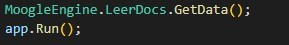
\includegraphics[width = 9cm]{img/MoogleServer.jpg}
        \caption[]{Fragmento de MoogleServer/Program.cs}
    \end{figure}

    \textbf{
            \\\large{LeerDocs:}\\
            \\
    }
    La clase estática \textbf{“LeerDocs”} contiene la función \textbf{“GetData()”} que utiliza la clase \textit{“Directory”}
    contenida en la biblioteca \textit{“System.IO”} para obtener un array con la dirección de todos 
    los archivos txt y luego lo recorro leyendo su contenido y creando un \textbf{“Vector”} por cada 
    documento
    \begin{figure}[h]
        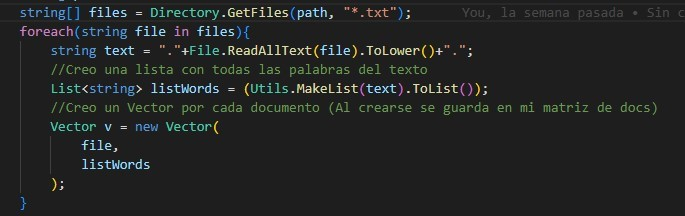
\includegraphics[width = 13cm]{img/LeerDocs.jpg}
        \caption[]{Función de GetData()}
    \end{figure}
    \textbf{
            \\\large{Vector:}\\
            \\
    }
    La clase \textit{Vector} tiene las siguientes propiedades:
    \begin{itemize}
        \item \textbf{TFIDF} (Dictionary$<$string, double$>$)
        \item \textbf{Path} (string)
        \item \textbf{Words} (List$<$string$>$)
    \end{itemize}
    \newpage
    \textbf{\\TFIDF:} Al crear un Vector se llama a la función \textit{“CountWords()”} que llena este diccionario con 
    la cantidad de veces que se repite cada palabra en el documento al que está asociado\\ \\
    \textbf{Path:} Al crear el vector de los documentos se le asigna la dirección del documento en la 
    computadora (desde el constructor).\\ \\
    \textbf{Words:} Contiene una lista con todas las palabras del documento.\\ \\
    \textbf{NOTA:} Al crear un vector, éste se guarda en la clase \textbf{Matriz}. \\ 

    \textbf{\\\large{Funciones de la clase Vector:}}
    \begin{itemize}
        \item  \textbf{CountWords()}
        \item \textbf{GetName()}
        \item  \textbf{ProdEscalar(Vector v)}
    \end{itemize}

    \textbf{CountWords():} Llena el \textit{Dictionary$<$string, double$>$ TFIDF} con la cantidad de veces que se repite cada palabra. Y 
    llena el \textit{Diccionario$<$string, int$>$ IDF} de la clase \textit{“Matriz”} con la cantidad de documentos en los 
    que aparece cada palabra del texto.\\
    (Ej: Si la palabra “hola” aparece en 5 docs, un elemento de \textit{Matriz.IDF} sería $<$hola, 5$>$).\\
    \textbf{CountWords():}GetName(): Obtiene el nombre del documento a partir de su \textit{Path}.\\
    \textbf{ProdEscalar(Vector v):} Se llama al realizar una query,
    \textit{(queryVector.ProdEscalar(anotherVector))}
    
    \begin{enumerate}
        \item Recorre las palabras de la query
        \item Calcula el TF-IDF de cada palabra de la query y lo guarda el Dictionary TFIDF
        \item Si el \textbf{Vector} “v” que recibe por parámetro contiene la palabra procede a calcular el TFIDF de dicha palabra en el vector
        \item Luego multiplica los TF-IDF de la palabra en cada \textbf{Vector} para así hallar el producto escalar entre ambos vectores 
    \end{enumerate}
    
    \textbf{
        \\\large{Matriz:}\\
        \\
    }
    La clase estática \textbf{Matriz} tiene las siguientes propiedades: 
    \begin{itemize}
        \item  \textbf{MatrizVectores}(List\textit{$<$Vector$>$})
        \item \textbf{IDF}(Dictionary\textit{$<$string, int$>$})
    \end{itemize}
    \textbf{MatrizVectores:} Cada vez que se crea un vector el mismo se agrega a esta lista de vectores 
    (Contiene todos los vectores de todos los documentos de la carpeta \textit{Content}). \\
    \textbf{IDF:} Al llamarse la función \textbf{CountWords()} de la clase \textbf{Vector} éste dictionary se llena con la 
    cantidad de documentos en los que aparece cada palabra del texto\\
    
    \textbf{
        \\\large{Funciones de la clase Matriz:}\\
        \\
    }
    
    \begin{itemize}
        \item  \textbf{Add}(Vector v)
        \item \textbf{CalculateIDF}(string w)
        \item \textbf{CalculateTF}(Vector v, string w)
    \end{itemize}
    \textbf{Add(\textnormal{Vector v}):} Agrega el vector “v” a \textbf{MatrizVectores}. \\
    \textbf{CalculateIDF(\textnormal{string w}):} Calcula el IDF de una palabra. Se usa al hacer el query por lo que ya 
    IDF contiene la cantidad de documentos en los que aparece cada palabra del texto.\\
    \textbf{CalculateTF(\textnormal{Vector v, string w}):} Calcula el IDF de una palabra. Se usa al hacer el query por 
    lo que ya v.TFIDF contiene la cantidad de veces que aparece la palabra en el texto.\\
    
    \textbf{
        \\\large{Search:}\\
        \\
    }
    La función \textbf{Search()} ubicada en la clase Moogle.cs retorna un array de \textbf{SearchItem}:
    
    \begin{enumerate}
        \item \textbf{Calcula el score} por cada vector y solo lo muestra si es mayor a $10^-6$ (Producto 
        escalar entre el query y el vector)
        \item Guarda la posición de la palabra con más TF-IDF del query que esté en el documento
        \item \textbf{Guarda el snippet} dado por un fragmento del texto que contenga dicha palabra
        (Desde punto (“.”) anterior a 50 caracteres antes de la palabra hasta el 
        siguiente punto después de 100 caracteres)
        Para ello se usan las funciones NextDot() y PrevDot() de mi clase Utils.
        \item Guarda en una Lista de SearchItem los datos del vector (nombre, snippet, score)
        \item Cuando termina de recorrer los vectores ordena la Lista de SearchItem según su score, 
        la convierte en Array y la devuelve    
    \end{enumerate}
    \textbf{
        \\\large{Utils:}\\
        \\
    }
    
    La clase estática \textbf{Utils} tiene las siguientes funciones:
    \begin{itemize}
        \item  \textbf{MakeList}(string text)
        \item \textbf{PrevDot}(int pos, string text)
        \item \textbf{NextDot}(int pos, string text)
    \end{itemize}
    \textbf{MakeList(\textnormal{string text}):} Convierte un string (text) en una \textit{List$<$string$>$} utilizando \textit{ToLower()} y
    \textit{Split()} sin caracteres especiales. \\
    \textbf{PrevDot(\textnormal{int pos, string text}):} Utilizando recursividad busca el punto anterior a la posición
    “pos” en el texto “text”.\\
    \textbf{NextDot(\textnormal{int pos, string text}):} Utiliza \textit{IndexOf(‘.’)} para saber la posición del siguiente punto 
    en el texto “text” luego de la posición “pos”.\\

\end{document}